%!TEX root =../mapp-challenge-18-game-book.tex
% ^ leave for LaTeXTools build functionality

\phChapterWorksheet{Blind Luck}{Cryptic Puzzle 3}

The Nickname Rater suggests you continue your journey down Road \(500\%\),
where an elusive \textbf{Dojo Master} is known to battle up-and-coming trainers.
You arrive at the dojo, but it seems that a secret password is required to
enter, and your only clue is the following image.

\newcommand{\blindCrissCrossEntry}[2]{
  \draw[step=1,dotted] #1 grid #2;
  \draw[very thick] #1 rectangle #2
}
\newcommand{\blindCrissCrossPip}[2]{
  \draw[fill=black] (#1.5,#2.5) circle (0.3)
}

\begin{center}
  RED BLUE YELLOW GOLD SILVER CRYSTAL

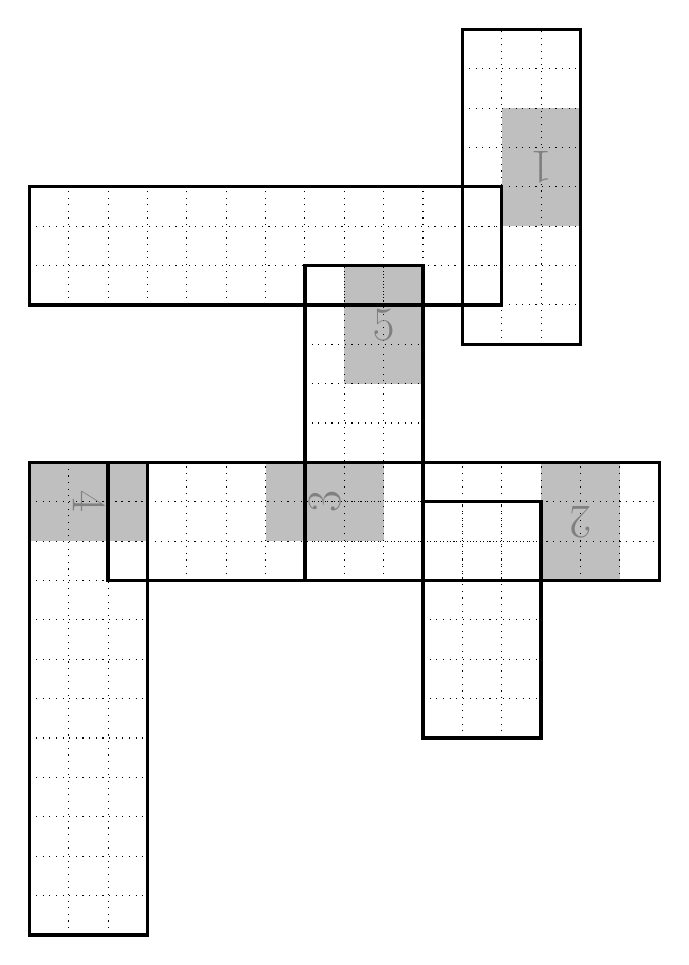
\begin{tikzpicture}[x=0.5cm,y=0.5cm]
  \fill[color=lightgray] (8,14) rectangle (10,17);
  \fill[color=lightgray] (0,10) rectangle (3,12);
  \fill[color=lightgray] (6,10) rectangle (9,12);
  \fill[color=lightgray] (13,9) rectangle (15,12);
  \fill[color=lightgray] (12,18) rectangle (14,21);

  \blindCrissCrossEntry{(0,0)}{(3,12)};
  \blindCrissCrossEntry{(2,9)}{(16,12)};
  \blindCrissCrossEntry{(10,5)}{(13,11)};
  \blindCrissCrossEntry{(7,9)}{(10,17)};
  \blindCrissCrossEntry{(0,16)}{(12,19)};
  \blindCrissCrossEntry{(11,15)}{(14,23)};

  \node at (9,15.5) {\LARGE\rotatebox{0}{\textcolor{gray}{5}}};
  \node at (1.5,11) {\LARGE\rotatebox{-90}{\textcolor{gray}{4}}};
  \node at (7.5,11) {\LARGE\rotatebox{90}{\textcolor{gray}{3}}};
  \node at (14,10.5) {\LARGE\rotatebox{180}{\textcolor{gray}{2}}};
  \node at (13,19.5) {\LARGE\rotatebox{180}{\textcolor{gray}{1}}};
\end{tikzpicture}
\end{center}

You'd move the \textbf{sun and moon} to figure out that password and battle the
Dojo Master! Calmly, you \textbf{shut your eyes} and begin to ponder the
solution to this mystery...


\phWorksheet{Solution}

\begin{center}
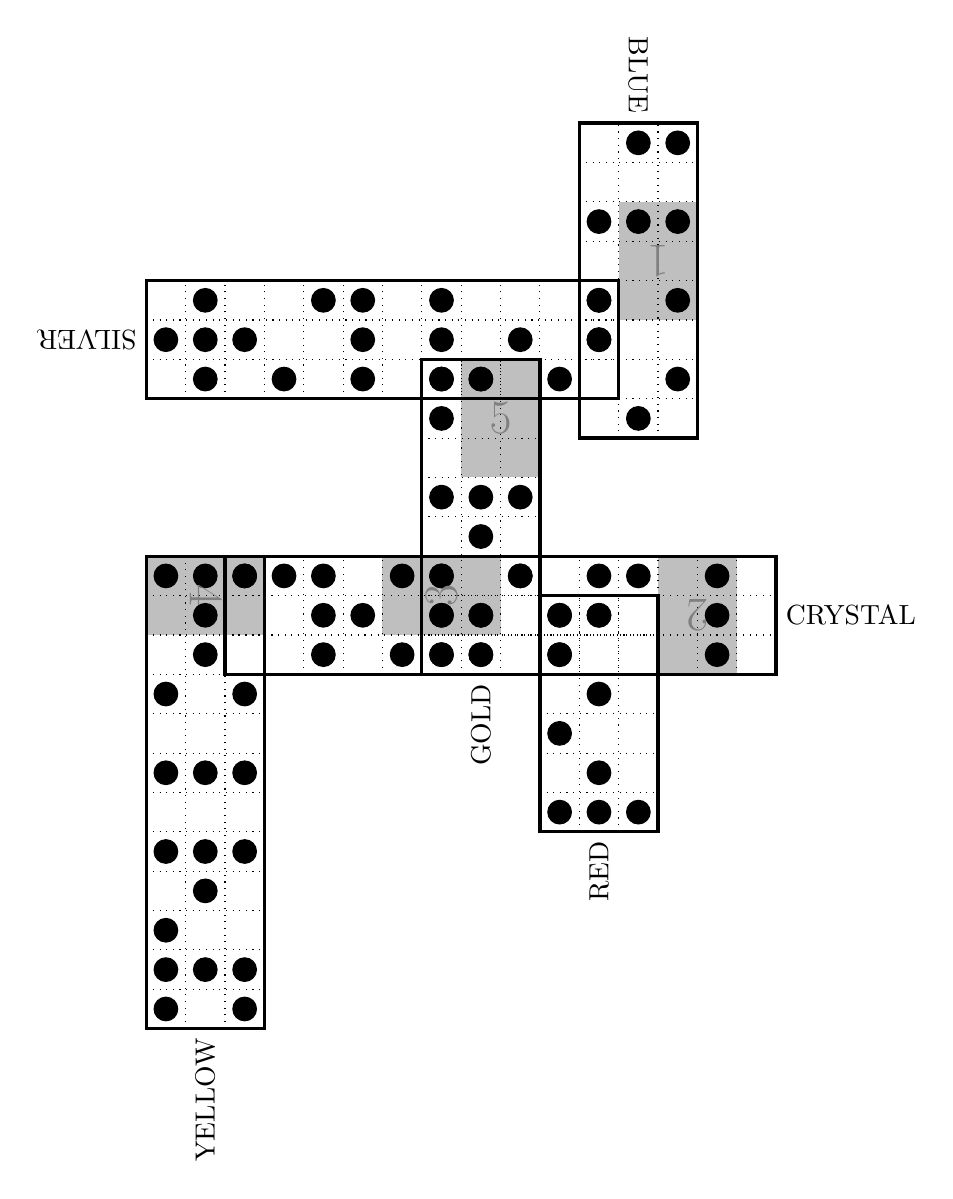
\begin{tikzpicture}[x=0.5cm,y=0.5cm]
  \fill[color=lightgray] (8,14) rectangle (10,17);
  \fill[color=lightgray] (0,10) rectangle (3,12);
  \fill[color=lightgray] (6,10) rectangle (9,12);
  \fill[color=lightgray] (13,9) rectangle (15,12);
  \fill[color=lightgray] (12,18) rectangle (14,21);

  \blindCrissCrossEntry{(0,0)}{(3,12)};
  \blindCrissCrossEntry{(2,9)}{(16,12)};
  \blindCrissCrossEntry{(10,5)}{(13,11)};
  \blindCrissCrossEntry{(7,9)}{(10,17)};
  \blindCrissCrossEntry{(0,16)}{(12,19)};
  \blindCrissCrossEntry{(11,15)}{(14,23)};

  %YELLOW
  \node[anchor=north] at (1.5,0) {\rotatebox{90}{YELLOW}};

  \blindCrissCrossPip{0}{0};
  \blindCrissCrossPip{2}{0};

  \blindCrissCrossPip{0}{1};
  \blindCrissCrossPip{1}{1};
  \blindCrissCrossPip{2}{1};

  \blindCrissCrossPip{0}{2};

  \blindCrissCrossPip{1}{3};

  \blindCrissCrossPip{0}{4};
  \blindCrissCrossPip{1}{4};
  \blindCrissCrossPip{2}{4};

  \blindCrissCrossPip{0}{6};
  \blindCrissCrossPip{1}{6};
  \blindCrissCrossPip{2}{6};

  \blindCrissCrossPip{0}{8};
  \blindCrissCrossPip{2}{8};

  \blindCrissCrossPip{1}{9};

  \blindCrissCrossPip{1}{10};

  \blindCrissCrossPip{0}{11};
  \blindCrissCrossPip{1}{11};
  \blindCrissCrossPip{2}{11};

  %CRYSTAL
  \node[anchor=west] at (16,10.5) {CRYSTAL};
  \blindCrissCrossPip{2}{11};

  \blindCrissCrossPip{3}{11};

  \blindCrissCrossPip{4}{9};
  \blindCrissCrossPip{4}{10};
  \blindCrissCrossPip{4}{11};

  \blindCrissCrossPip{5}{10};

  \blindCrissCrossPip{6}{9};
  \blindCrissCrossPip{6}{11};

  \blindCrissCrossPip{7}{9};
  \blindCrissCrossPip{7}{10};
  \blindCrissCrossPip{7}{11};

  \blindCrissCrossPip{8}{9};
  \blindCrissCrossPip{8}{10};

  \blindCrissCrossPip{9}{11};

  \blindCrissCrossPip{10}{9};
  \blindCrissCrossPip{10}{10};

  \blindCrissCrossPip{11}{10};
  \blindCrissCrossPip{11}{11};

  \blindCrissCrossPip{12}{11};

  \blindCrissCrossPip{14}{9};
  \blindCrissCrossPip{14}{10};
  \blindCrissCrossPip{14}{11};

  %RED
  \node[anchor=north] at (11.5,5) {\rotatebox{90}{RED}};

  \blindCrissCrossPip{10}{5};
  \blindCrissCrossPip{11}{5};
  \blindCrissCrossPip{12}{5};

  \blindCrissCrossPip{11}{6};

  \blindCrissCrossPip{10}{7};

  \blindCrissCrossPip{11}{8};

  \blindCrissCrossPip{10}{9};

  \blindCrissCrossPip{10}{10};
  \blindCrissCrossPip{11}{10};

  %GOLD
  \node[anchor=north] at (8.5,9) {\rotatebox{90}{GOLD}};

  \blindCrissCrossPip{7}{9};
  \blindCrissCrossPip{8}{9};

  \blindCrissCrossPip{7}{10};
  \blindCrissCrossPip{8}{10};

  \blindCrissCrossPip{7}{11};
  \blindCrissCrossPip{9}{11};

  \blindCrissCrossPip{8}{12};

  \blindCrissCrossPip{7}{13};
  \blindCrissCrossPip{8}{13};
  \blindCrissCrossPip{9}{13};

  \blindCrissCrossPip{7}{15};

  \blindCrissCrossPip{7}{16};
  \blindCrissCrossPip{8}{16};

  %SILVER
  \node[anchor=east] at (0,17.5) {\rotatebox{180}{SILVER}};

  \blindCrissCrossPip{11}{18};
  \blindCrissCrossPip{11}{17};

  \blindCrissCrossPip{10}{16};

  \blindCrissCrossPip{9}{17};

  \blindCrissCrossPip{8}{16};

  \blindCrissCrossPip{7}{18};
  \blindCrissCrossPip{7}{17};
  \blindCrissCrossPip{7}{16};

  \blindCrissCrossPip{5}{18};
  \blindCrissCrossPip{5}{17};
  \blindCrissCrossPip{5}{16};

  \blindCrissCrossPip{4}{18};

  \blindCrissCrossPip{3}{16};

  \blindCrissCrossPip{2}{17};

  \blindCrissCrossPip{1}{18};
  \blindCrissCrossPip{1}{17};
  \blindCrissCrossPip{1}{16};

  \blindCrissCrossPip{0}{17};

  %BLUE
  \node[anchor=south] at (12.5,23) {\rotatebox{-90}{BLUE}};

  \blindCrissCrossPip{12}{22};
  \blindCrissCrossPip{13}{22};

  \blindCrissCrossPip{11}{20};
  \blindCrissCrossPip{12}{20};
  \blindCrissCrossPip{13}{20};

  \blindCrissCrossPip{11}{18};
  \blindCrissCrossPip{13}{18};

  \blindCrissCrossPip{11}{17};

  \blindCrissCrossPip{13}{16};

  \blindCrissCrossPip{12}{15};

  \node at (9,15.5) {\LARGE\rotatebox{0}{\textcolor{gray}{5}}};
  \node at (1.5,11) {\LARGE\rotatebox{-90}{\textcolor{gray}{4}}};
  \node at (7.5,11) {\LARGE\rotatebox{90}{\textcolor{gray}{3}}};
  \node at (14,10.5) {\LARGE\rotatebox{180}{\textcolor{gray}{2}}};
  \node at (13,19.5) {\LARGE\rotatebox{180}{\textcolor{gray}{1}}};
\end{tikzpicture}
\end{center}

The numbered regions spell out \texttt{ULTRA} in Braille.


% Include below for aucTeX integration
%%% Local Variables:
%%% mode: latex
%%% TeX-master: "../mapp-challenge-18-game-book"
%%% End:
